\chapter{Overview of Pattern Recognition Techniques}

In this chapter, we will discuss the mathematical foundations of the patern recognition methods that will be used to predict 
scores. There are two approaches to this. The first is to use already built packages for both a given programming language and simply
feed data into it and present the results. The second method is to build them from scratch. The disadvantage to doing this is naturally 
that it is more time consuming. However, it does allow for more control over how our models work, and will allow us to understand our results
better, than if we had used a proprietary model. This isn't to say that the code written for these models won't utilise packages for doing things
like linear algebra calculations, but we wont simply import a neural network package and have results within 5 lines of code. \\

%Explain which langauges were chosen for each method and why


\section{Neural Networks}

\subsection{A Brief Introduction to Neural Networks}
Neural networks (NNs) have been the subject to a lot of hype in recent years. They are a machine learning method that is being applied to many problems
in all sorts of fields.  %some references here please 
The network will be trained on runrate data, so for each game we have calculated the evolution of the runrate,
and then we have the overall score for that game in the final column of the matrix. An example of a network can be seen in \ref{nnexample1}. The first layer is the 
input layer, and the last layer gives the predictions. The middle layers are hidden and where the work of the network is done. \\

Let's look at what a NN actually looks like. The below is an example of a network with just one hidden layer.

\begin{figure}
    \centering
    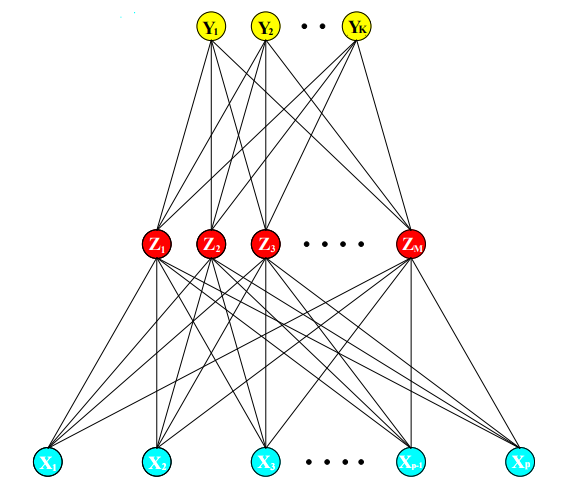
\includegraphics[scale=0.5]{figures/nn.png}
    \caption{Example of a single hidden layer neural network, as in \cite{sprbk}}
    \label{nnexample1}
\end{figure}

We see there are $p$ input nodes at the bottom, M nodes in the hidden layer, and K output layers. The lines between the layers are given a ``weight''
and a ``bias''. These properties will be discussed in more detail shortly. The number of hidden layers to be used will be the subject of experimentation. In order to find try this out, we will have to randomly
split the matrix into a training matrix and a testing matrix. We can then evaluate the network by trying to predict values from the testing set and seeing
how well it does. This will then lead to us refining the number of hidden layers as appropriate. \\

One area of the world where neural networks are being applied to value prediction is in the stock market. Naturally if one can predict how the value of a stock
will change over some time period, then one can protect themself from a bad investment, or profit heavily from a good one. We will use similar
methods here for building our neural network.  In \cite{nnstock}, the authors twest two different Neural Netowrks, and find that using a ``Multi-Layer Feed Forward Nerual Network''
is the better choice for predicting how stock values will change. With these motivations in mind, we can begin to construct the networks.

\subsection{Builiding The Network}
Our input layer will have 50 nodes, one for the runrate at the end of each over. We will begin with 5 hidden layers, although this is subject to change. The output layer
will of course only have one node, the value of which will predict the score of the game. 

We begin by looking at a single node. The proper name for each node is ``perceptron''. Each perceptron takes in the values of a vector, and an extra ``+1'' intercept term. The perceptron then outputs a valye h given by \ref{percepout}:

\begin{equation}
    \label{percepout}
    h_{W,b}(x) = f(\textbf{W}^Tx) = f(\sum_{i=1}^KW_ix_i+b).
\end{equation}

Here, $K \in \mathbb{N}$ is the number of elements in the vector, and $f:\mathbb{R} \rightarrow \mathbb{R}$ is called the activation function. There is a bit of choice in which activation function to use.
The two common choices are:

\begin{align}
    f(z) &= \frac{1}{1+exp(-z)} \\
    f(z) &= tanh(z)
\end{align}

The comparrison of these two functions can be seen in \red{actfig}.

\begin{figure}[h]
    \centering
    \label{actfig}
    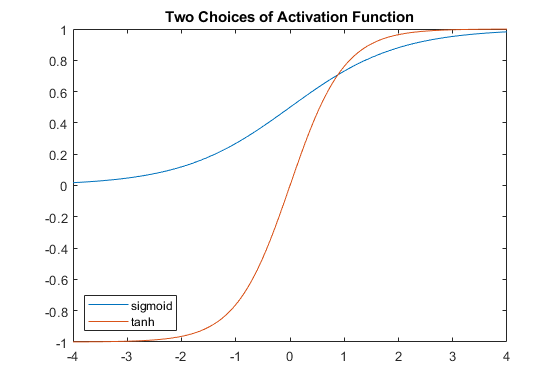
\includegraphics[scale=0.5]{figures/actfuncs.png}
    \caption{Graph showing the shape of different activation functions.}
\end{figure}

We will be using (4.2) as our activation, known as the ``sigmoid function''. 